%!TEX root = ../template.tex
%%%%%%%%%%%%%%%%%%%%%%%%%%%%%%%%%%%%%%%%%%%%%%%%%%%%%%%%%%%%%%%%%%%%
%% chapter3.tex
%% NOVA thesis document file
%%
%% Chapter with a short latex tutorial and examples
%%%%%%%%%%%%%%%%%%%%%%%%%%%%%%%%%%%%%%%%%%%%%%%%%%%%%%%%%%%%%%%%%%%%

\typeout{NT FILE chapter3.tex}%
\chapter{Preliminary Work}

This chapter presents the initial experiments using machine learning for breast
cancer molecular subtype classification based on the patients’ microRNAs
expression levels. Early work focused on testing baseline \gls{ml} models
(Logistic Regression, SVM, Random Forest) to assess their classification
performance using datasets such as TCGA-BRCA \cite{TCGA_BRCA}.

\section{Dataset and Pre-processing}
The dataset utilized in this study is derived from the Cancer Atlas Program
(TCGA), a widely recognized and reliable source of this particular type of
data. The TCGA-BRCA project provides researchers with access to a comprehensive
set of data and resources, including microRNA expression profiles associated
with breast cancer patients, gene expression data, clinical data, and
additional data from various sources. As demonstrated in Table
\ref{tab:dataset_description}, this dataset poses significant challenges,
primarily concerning its dimensionality, class imbalance, redundancy of
microRNA expression values, and feature names. The absence of standardized
naming guidelines for miRNAs further complicates this issue. For instance, a
miRNA may be designated as "\textit{hsa-mir-145}" or "\textit{MIR-145},"
necessitating the incorporation of a "translation" layer during the
pre-processing stage to ensure compatibility with data from external projects
or repositories.

\begin{table}[h]
  \centering
  \caption{Dataset Description wtih the number of samples, microRNAs expression features, and clinical attributes before and after pre-processing.}

  \begin{tabular}{|l|l|l|l|}
    \hline
    \textbf{Statistics}  & \textbf{Before pre-processing} & \textbf{After pre-processing} \\ \hline
    \# Samples           & 463                            & 256                           \\ \hline
    \# miRNAs            & 888                            & 442 \footnotemark[1]          \\ \hline
    \# Clinical Features & 22                             & 20                            \\ \hline
    \# Classes           & 5                              & 4 \footnotemark[1]            \\ \hline
    % Add more rows as needed
  \end{tabular}
  \label{tab:dataset_description}
\end{table}

\footnotetext[1]{Only applied in the second part of the tests, more details in \ref{sec:second_segment}}

During the data preparation phase, we eliminated features that had more over
60\% of missing values and, additionally, the "Normal-like" class due to its
limited sample size of only five instances, which is insufficient for training
a reliable model. In terms of samples, there was a few samples with missing
values in some miRNAs and clinical features, which were removed from the
dataset to prevent the use of SMOTE or other imputation methods that could
introduce bias or noise into the data. Even though we have 888 different miRNA
features, there are some columns that are duplicates of others - why? well,
let’s consider the base \textit{MIR-16} as an example, this miRNA has 6
different forms of expression: \textit{MIR-16/3P, MIR-16/16, MIR-16/5P,
  MIR-16-1/16, MIR-16-13/16, MIR-16-2/16} -, all of these have the same values
because the extraction technique that was used to obtain the miRNA expression
values is not sensitive enough to detect the differences. Given that, to remove
redundancy, we decided to remove all miRNAs that share the same base, ending up
with 442 miRNAs. Regarding the contextual importance of features, there are
some features (i.e. study Id) that were neither important, nor their values had
much variance, which would not benefit the model. Adding to all of this, I
mapped the categorical features to numerical values to ensure that the models
could process them correctly. The table provides a summary of the dataset after
pre-processing, including the number of samples, features, and clinical
attributes.

\section{First tests with baseline models}

Given the reduced data set, we did an initially split of 80\% for training and
20\% for testing, with no validation set. The models were trained using the
\textit{scikit-learn} library, and the results were evaluated using accuracy,
precision, recall, and F1-score metrics. First, I evaluated the quality of the
split using a 2D Projection of the data using Principal Component Analysis
(PCA) wiht k = 2 PCA is a dimensionality reduction technique that transforms
the data into a lower dimensional space while preserving the variance of the
data. The PCA projection is shown in Figure \ref{fig:side_by_side_pca}. The PCA
projection shows that the training and testing sets are well mixed, indicating
that the split is representative of the data. For this evaluation, I also
plotted the proportion of each class in the training and testing sets, as shown
in Figure \ref{fig:baseline_class_proportions}, which indicates that the split
is balanced and representative of the data.

\begin{figure}[ht]
  \centering
  \begin{subfigure}[t]{0.48\textwidth}
    \centering
    \includegraphics[width=\textwidth]{/Users/JoseRomano/Documents/Tese/bca-thesis/Chapters/Figures/pca1.png}
    \caption{}
    \label{fig:baseline_pca_projection1}
  \end{subfigure}
  \hfill
  \begin{subfigure}[t]{0.48\textwidth}
    \centering
    \includegraphics[width=\textwidth]{/Users/JoseRomano/Documents/Tese/bca-thesis/Chapters/Figures/pca2.png} % <-- Update this path to your second image
    \caption{}
    \label{fig:baseline_pca_projection2}
  \end{subfigure}
  \caption{(a) PCA projection of the training and testing sets. The colors represent the different sets, and the points represent the samples. (b) Same PCA projection, but with the classes represented by different colors.}
  \label{fig:side_by_side_pca}
\end{figure}

\definecolor{customblue}{RGB}{121,168,201}
\definecolor{customorange}{RGB}{255,180,112}

\begin{figure}
  \centering
  \resizebox{0.4\linewidth}{!}{
    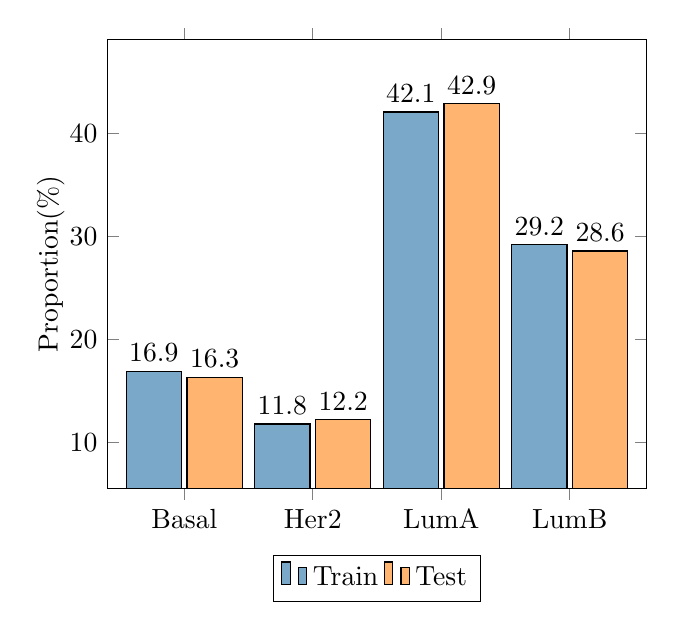
\begin{tikzpicture}
      \begin{axis}[
          ybar,
          enlargelimits=0.2,
          legend style={at={(0.5,-0.15)},
              anchor=north,legend columns=-1},
          ylabel={Proportion(\%)},
          ylabel style={yshift=-5pt},
          symbolic x coords={Basal, Her2, LumA, LumB},
          xtick=data,
          nodes near coords,
          nodes near coords align={vertical},
          bar width=20pt,
        ]

        % Dados de treino
        \addplot[fill=customblue] coordinates {(Basal,16.9) (Her2,11.8) (LumA,42.1) (LumB,29.2)};

        % Dados de teste
        \addplot[fill=customorange] coordinates {(Basal,16.3) (Her2,12.2) (LumA,42.9) (LumB,28.6)};

        \legend{Train, Test}
      \end{axis}
    \end{tikzpicture}
  }
  \caption{Class proportions in the training and testing sets. The colors represent the different sets, and the bars represent the proportion of each class.}
  \label{fig:baseline_class_proportions}
\end{figure}

After the split, I trained three baseline models: Logistic Regression, XGBoost,
and Naive Bayes. The results of the models are shown in Table
\ref{tab:baseline_models_results}.

\begin{table}
  \centering
  \caption{Results of the baseline models on the testing set. The table shows the precision, recall, F1-score, and support for each class, as well as the overall accuracy of the models.}
  \label{tab:baseline_models_results}
  \resizebox{0.8\textwidth}{!}{
    \begin{tabular}{llrrrr}
      \toprule
      \textbf{Model} & \textbf{Class}            & \textbf{Precision}       & \textbf{Recall} & \textbf{F1-score} & \textbf{Support} \\
      \midrule
      \multirow{4}{*}{Random Forest}
                     & 0                         & 0.89                     & 1.00            & 0.94              & 8                \\
                     & 1                         & 1.00                     & 0.17            & 0.29              & 6                \\
                     & 2                         & 0.64                     & 0.76            & 0.70              & 21               \\
                     & 3                         & 0.50                     & 0.50            & 0.50              & 14               \\
      \cmidrule{2-6}
                     & \textit{Overall Accuracy} & \multicolumn{4}{r}{0.65}                                                          \\
      \midrule
      \multirow{4}{*}{XGBoost}
                     & 0                         & 1.00                     & 1.00            & 1.00              & 8                \\
                     & 1                         & 0.75                     & 0.50            & 0.60              & 6                \\
                     & 2                         & 0.86                     & 0.90            & 0.88              & 21               \\
                     & 3                         & 0.73                     & 0.79            & 0.76              & 14               \\
      \cmidrule{2-6}
                     & \textit{Overall Accuracy} & \multicolumn{4}{r}{0.84}                                                          \\
      \midrule
      \multirow{4}{*}{Naive Bayes}
                     & 0                         & 0.80                     & 1.00            & 0.89              & 8                \\
                     & 1                         & 0.40                     & 0.33            & 0.36              & 6                \\
                     & 2                         & 0.79                     & 0.52            & 0.63              & 21               \\
                     & 3                         & 0.45                     & 0.64            & 0.53              & 14               \\
      \cmidrule{2-6}
                     & \textit{Overall Accuracy} & \multicolumn{4}{r}{0.61}                                                          \\
      \bottomrule
    \end{tabular}
  }
\end{table}

\section{Second Segment of Experiments}
\label{sec:second_segment}

In this section, I re-processed the dataset from scratch to ensure a clean and
leakage-free setup. Given the concerns raised about the normalization
procedures in the first segment, I implemented a more robust pre-processing
pipeline to address these issues. The new pipeline includes the following
steps:
\begin{enumerate}
  \item Removal of features with more than 60\% missing values.
  \item Removal of the "Normal-like" class due to its limited sample size.
  \item Removal of redundant miRNAs based on their base names.
  \item Removal of features that were neither important nor had much variance.
  \item Mapping of categorical features to numerical values.
\end{enumerate}

Then, I split the dataset into training and testing sets using an 80/20 split,
ensuring that the split is representative of the data. Only after the split, I
applied normalization to the training set using the \textit{StandardScaler}
from the \textit{scikit-learn} library. The normalization was then applied to
the testing set using the same scaler fitted on the training set. This approach
ensures that the normalization is consistent across the training and testing
sets, preventing data leakage. A scaler is the mean and standard deviation of
the training set, which is then used to normalize the testing set. This
approach ensures that the testing set is not used to fit the scaler, preventing
data leakage. The formula used for normalization, from
\textcite{sklearn_normalization}.

% \[
%   z = \frac{x - \mu}{\sigma}
% \]

% where:
% \begin{itemize}
%   \item \( x \) is the original value,
%   \item \( \mu \) is the mean of the feature,
%   \item \( \sigma \) is the standard deviation of the feature,
%   \item \( z \) is the standardized value.
% \end{itemize}

With this new pre-processing pipeline, I re-ran the same baseline models and
leveraged the use of greater computational resources for hyperparameter tuning
using a grid search approach. These efforts showed that XGBoost outperformed
any other model tested, including latent space models such as \textit{DIABLO}.

\begin{table}
  \centering
  \caption{Results of the heterogeneous models (miRNAs + Clinical Data) on the testing set. The table shows overall performance and F1-score per class.}
  \label{tab:heterogeneous_models_results}
  \resizebox{0.8\textwidth}{!}{
    \begin{tabular}{llrrrr}
      \toprule
      \textbf{Model} & \textbf{Class} & \textbf{Precision} & \textbf{Recall} & \textbf{F1-score} & \textbf{Ovr. Accuracy}     \\
      \midrule
      \multirow{4}{*}{DIABLO All Blocks}
                     & Basal          & 1.00               & 1.00            & 1.00              & \multirow{4}{*}{0.80} \\
                     & HER2           & 0.50               & 0.33            & 0.40              &                       \\
                     & Luminal A      & 0.75               & 1.00            & 0.86              &                       \\
                     & Luminal B      & 0.89               & 0.57            & 0.70              &                       \\
      \midrule
      \multirow{4}{*}{Decision Tree}
                     & Basal          & 0.80               & 1.00            & 0.89              & \multirow{4}{*}{0.61} \\
                     & HER2           & 0.60               & 0.50            & 0.55              &                       \\
                     & Luminal A      & 0.62               & 0.62            & 0.62              &                       \\
                     & Luminal B      & 0.46               & 0.43            & 0.44              &                       \\
      \midrule
      \multirow{4}{*}{Logistic Regression}
                     & Basal          & 1.00               & 0.88            & 0.94              & \multirow{4}{*}{0.80} \\
                     & HER2           & 0.67               & 0.67            & 0.55              &                       \\
                     & Luminal A      & 0.90               & 0.86            & 0.87              &                       \\
                     & Luminal B      & 0.63               & 0.71            & 0.67              &                       \\
      \midrule
      \multirow{4}{*}{XGBoost}
                     & Basal          & 1.00               & 1.00            & 1.00              & \multirow{4}{*}{0.84} \\
                     & HER2           & 1.00               & 0.67            & 0.67              &                       \\
                     & Luminal A      & 0.83               & 0.95            & 0.85              &                       \\
                     & Luminal B      & 0.85               & 0.79            & 0.77              &                       \\
      \bottomrule
    \end{tabular}
  }
\end{table}

The comparison between baseline models (trained on potentially leaked data) and
heterogeneous models (trained on properly preprocessed data with clinical
features) shows a clear improvement in model generalizability and robustness.

In the first setup, XGBoost achieved high performance (accuracy = 84\%), but
likely benefited from data leakage. Once the pipeline was corrected, all models
showed more realistic and balanced results. XGBoost remained the top performer
(accuracy = 84\%, F1 = 1.00 for Basal-like, 0.85 for Luminal A, and 0.77 for
Luminal B), while Logistic Regression also performed well (accuracy = 80\%).

However, HER2-enriched and Luminal B subtypes consistently showed lower
F1-scores across models. This bottleneck is likely due to their low
representation in the dataset and the biological similarity of their miRNA
expression profiles, which reduces class separability and hampers learning.

Overall, the results confirm the importance of careful preprocessing and the
benefit of integrating clinical data, especially for improving performance on
harder-to-distinguish subtypes.

